\section{Inhalte hinzufügen}
\frame{
    \frametitle{Inhalte hinzufügen}
	Artikel sind dezentral im Zuständigkeitsbereich abzulegen, d.h. im passenden Ordner des Bereiches.
	Generell ist die zentrale Ablage von z.B. Nachrichten unter ``news'' zu vermeiden. 
    Artikeltypen:
    \begin{itemize}
        \item Ordner
        \item Bild
        \item Seite
        \item Datei
        \item Link
        \item Termin
        \item Nachricht
        \item Kollektion
    \end{itemize}
}
\frame{
    \frametitle{Inhalte hinzufügen}
    \begin{figure}[!h]
        \centering
    %\begin{wrapfigure}{r}{0.4\textwidth}
        %\vspace{-20pt}
        %\begin{center}
            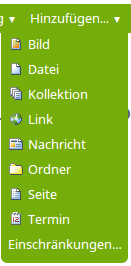
\includegraphics[width=0.33\textwidth]{../res/artikel-hinzufuegen.png}
        %\vspace{-20pt}
        %\end{center}
        \caption{Artikeltyp hinzuf\"ugen}
    %\end{wrapfigure}
    \end{figure}
}


\subsection{Kategorisierung}
\frame{
    \frametitle{Kategorisierung}
   \begin{itemize}
	\item Nicht persönliche Artikel jeden Typs sollten so umfangreich wie möglich kategorisiert werden. 
	\item Durch die Kategorisierung tauchen die Artikel in entsprechen Kollektionen auf
   \end{itemize}
   \begin{hinweis}
   \item Mehrere Stichworte müssen mit gedrückter \textit{Strg}-Taste ausgewählt werden.
   \end{hinweis}
    \begin{figure}[!h]
        \centering
        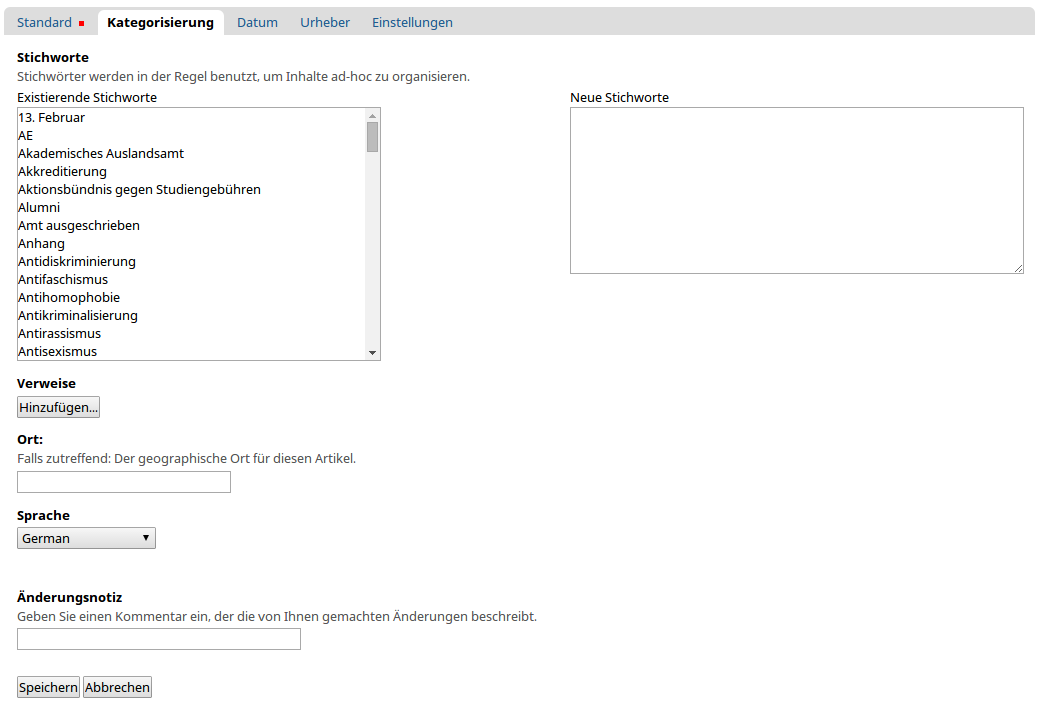
\includegraphics[width=0.66\textwidth]{../res/stura-kategorien.png}
    \end{figure}
}


\subsection{Artikeltypen}
\frame{
    \frametitle{Artikeltyp - Ordner}
    \begin{itemize}
        \item Angaben: Name, Titel, Beschreibung
        \item Startartikel: index\_html, index.html, index.htm, FrontPage
        \item Ansicht ändern
    \end{itemize}
    % Erweitertes Wissen
    %Darüberhinaus sind für Ordner noch weitere Aktionen möglich:
    %\begin{itemize}
    %    \item Syndikation
    %    \item Lokale Rollen
    %\end{itemize}
    \begin{figure}[!h]
        \centering
        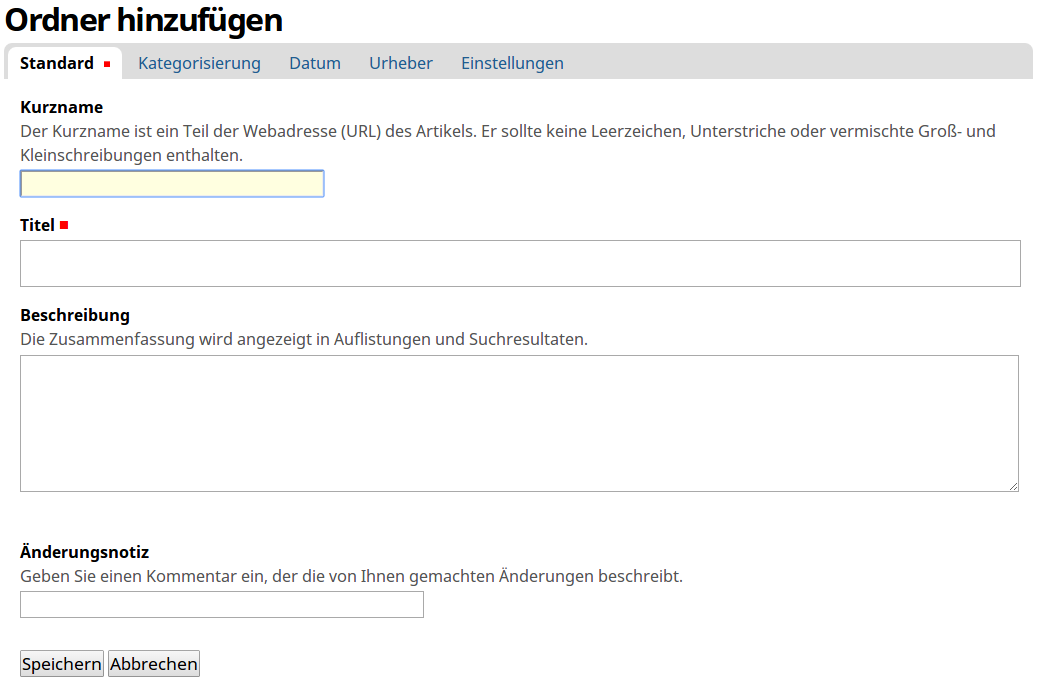
\includegraphics[width=0.75\textwidth]{../res/ordner-hinzufuegen.png}
    \end{figure}
}

\frame{
    \frametitle{Artikeltyp - Bild}
    Anschließend öffnet sich das folgende Formular:
    \begin{figure}[!h]
        \centering
        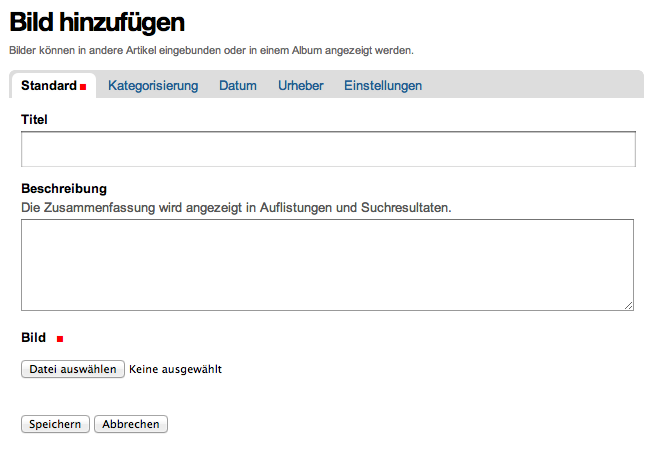
\includegraphics[width=\textwidth]{../res/bild-hinzufuegen_2.png}
    \end{figure}
}
\frame{
    \frametitle{Artikeltyp - Bild}
    \begin{description}
        \item[Titel] Aus dem Titel wird der Kurzname oder ID des Artikels gebildet.
 Wird kein Titel angegeben, behält das Bild üblicherweise seine ursprüngliche
 ID bei.

        \item[Beschreibung] Diese wird unter anderem bei der Anzeige von Suchergebnissen verwendet.

        \item[Bild] Klicken Sie auf *Datei auswählen* um auf Ihrem lokalen Computer eine Bilddatei zum Hochladen auszuwählen.
     Sie sollten die Bilder vor dem Auswählen für die Verwendung im Web
     vorbereiten. Eine kurze Anleitung hierzu finden Sie in `Bilder optimieren
     %<bilder-optimieren.html>`\_.

     Nach dem Hochladen wird Ihnen dann eine Vorschau des Bildes angezeigt.
        \item[Stichworte] Da Bilder nicht textuell erschlossen werden können, kommt den Stichworten eine besondere Bedeutung zu.
    \end{description}
}

\frame{
    \frametitle{Artikeltyp - Bild}
 \begin{tip}
     \item Eine Einführung zur Verschlagwortung von Bildern finden Sie unter
 `Verschlagwortungsstrategien
 \url{https://www.veit-schiele.de/profil/artikel/verschlagwortungsstrategien}`
 \end{tip}
}

\frame{
    \frametitle{Artikeltyp - Seite}
    \begin{itemize}
        \item Angaben: Name, Titel, Beschreibung, Eigenschaften
        \item Inhalte via Webbrowser eingebar
    \end{itemize}
    Dabei kann der Text in folgenden Formaten eingegeben werden:
    \begin{description}
        \item[HTML] ermöglicht Ihnen die direkte Eingabe von HTML;
        \item[Einfacher Text] ermöglicht Ihnen die einfache Eingabe von Text.
        \item[Markdown] ermöglicht Ihnen die direkte Eingabe mit Markdown-Syntax
    \end{description}

    Optional können Sie auch Textdateien auf den Server hochladen.
}

\frame{
    \frametitle{Artikeltyp - Datei}

	Dateiobjekte können Dateien enthalten, die heruntergeladen werden können.
	Hinzufügen:
	\begin{itemize}
	\item ``Durchsuchen\dots''-Taste klicken
	\item Verzeichnis durchsuchen, Datei auswählen
	\item ``Hochladen\dots''-Taste klicken
	\end{itemize}
	Die Bezeichnung, Beschreibung und Kategorisierung der Datei sind sehr relevant, da nur durch sie das einfache Auffinden der Datei gewährleistet werden kann.
    \begin{figure}
    %\begin{wrapfigure}{o}{\textwidth}
        %\vspace{-20pt}
        %\begin{center}
            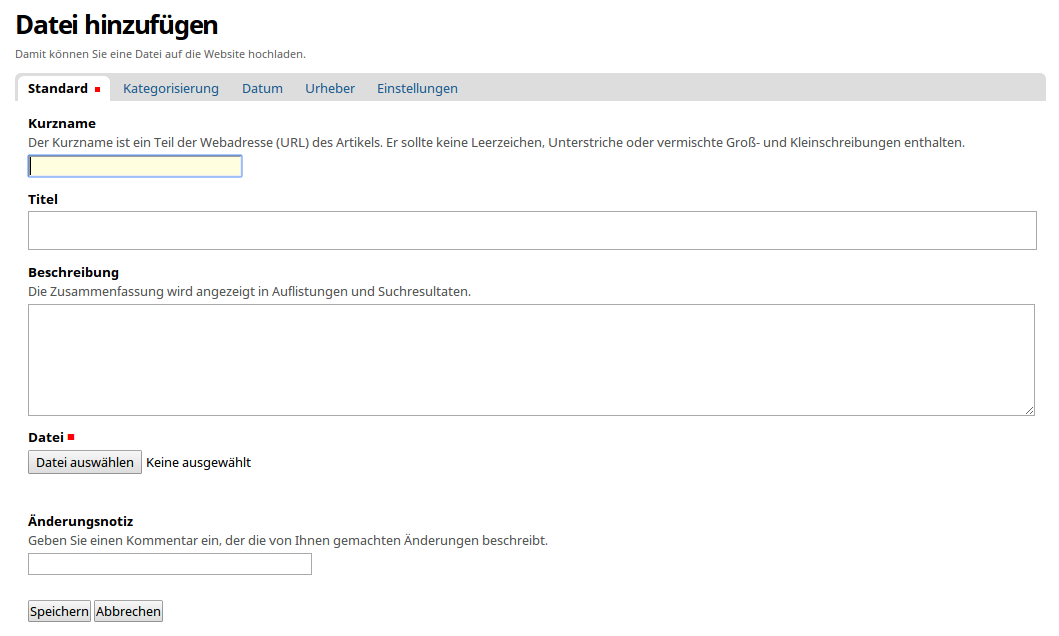
\includegraphics[width=0.5\textwidth]{../res/datei-hinzufuegen.png}
        %\vspace{-20pt}
        %\end{center}
        \caption{Datei hinzuf\"ugen}
    %\end{wrapfigure}
    \end{figure}
}

\frame{
    \frametitle{Artikeltyp - Link}
Links können als Schnellverweise gesetzt werden. 
So führt z.B. der Link \url{www.stura.htw-dresden.de/ese} für Externe direkt auf den Ordner der ESE. 
    Bitte beachten Sie bei der Angabe von externen Links die Angabe des Protokolls (z.B. ``http://'' für Webpages oder ``ftp://'' für Dateien).

    %\begin{tip}
     %   \item Auch eine Suchanfrage können Sie einfach speichern indem Sie einen Link mit der URL der Suchergebnisse erzeugen – bei jedem Aufruf des Links wird dann die Suchanfrage erneut gestartet.
    %\end{tip}

}

\frame{
    \frametitle{Artikeltyp - Termin}
    Termine sind Objekte, die im Kalender eingetragen werden. Termine sollten im Ordner \textit{Termine} der ``zuständigsten'' Stelle, z.B Referat, Bereich oder Projekt eingetragen werden. Grundsätzlich sollten Termine von der Navigation ausgeschlossen werden. Dazu ist beim Artikel über Bearbeiten und Einstellungen ein Haken bei ``Von Navigation ausschließen'' zu setzen.

    \begin{itemize}
        \item Angabe: Name, Titel, Beschreibung
        \item weiter Ereignistypen, die auch als Schlagwörter verwendet werden
    \end{itemize}
    \begin{hinweis}
        \item Wollen Sie die Einträge in dieser Liste geändert haben, wenden Sie sich bitte an die Administration der Website.
    \end{hinweis}
}

\frame{
    \frametitle{Artikeltyp - Termin}
    \begin{description}
        \item[Terminanfang] Datum und Uhrzeit des Beginns; Sie können alternativ auch im nebenstehenden Kalender den Beginn auswählen.
        \item[Terminende] Datum und Uhrzeit können alternativ auch in nebenstehendem Kalender angegeben werden.
        \item[Terminort] Hier können Sie den Ort des Termins angeben.
        \item[Terminankündigung] Ankündigungstext für den Termin; alternativ können Sie auch eine Textdatei hochladen.
        \item[Teilnehmer] Teilnehmende des Termins.
        \item[Terminart] Die Art des Termins.
        \item[URL] Hier können Sie eine Web-Adresse angeben, die weitergehende Informationen über dieses Ereignis liefert.
        \item[Kontaktname] Kontaktperson oder -organisation für das Ereignis.
        \item[Kontaktadresse] Adresse, bei der Sie weitergehende Informationen zum Ereignis erhalten können.
        \item[Kontakt-E-Mail] E-Mail-Adresse für Nachfragen.
        \item[Kontakt-Telefon] Telefonnummer für Nachfragen und Reservierungen.
    \end{description}
}

\frame{
    \frametitle{Artikeltyp - Nachricht}
    Nachrichten sind Seiten  mit Titel, optionaler Beschreibung und Bild.

    Für Nachrichten lassen sich im Gegensatz zu Seiten noch je ein Bild mit Bildtitel angeben.
    \begin{figure}[!h]
        \centering
        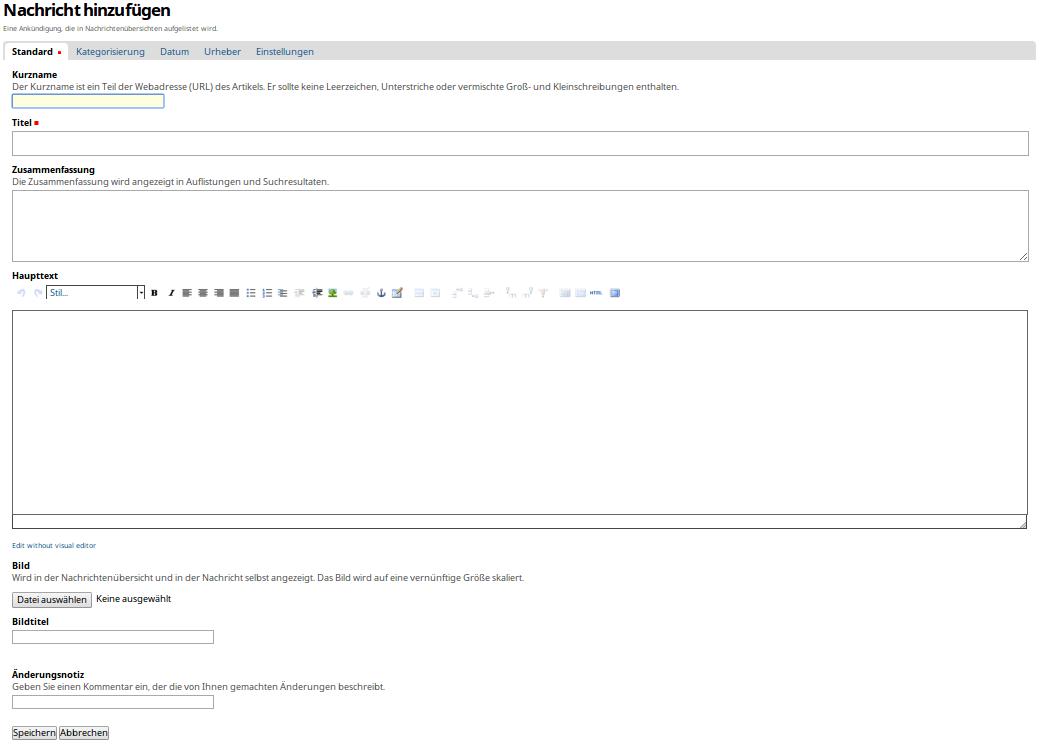
\includegraphics[width=0.75\textwidth]{../res/nachricht-hinzufuegen.png}
    \end{figure}
}

\frame{
    \frametitle{Artikeltyp - Kollektion}
    Kollektionen sind vorgefertigte Suchanfragen, die auch die Erschließung großer Datenbestände erlauben.

Kollektionen können üblicherweise nicht von allen Mitgliedern eines Portals hinzugefügt werden, sondern nur von denjenigen, die die Rollen *Website-Administrator* oder *Verwalter* innehaben. siehe: \url{www.stura.htw-dresden.de/stura/ref/verwaltung}
}

%\frame{
%    \frametitle{Artikeltyp - Kollektion}
%    \begin{figure}[!h]
%        \centering
%        \includegraphics[width=0.66\textwidth]{../res/kollektion-hinzufuegen.png}
%    \end{figure}
%   Hinzufügen-Menü mit ausgewählter Kollektion
%}
%
%\frame{
%    \frametitle{Artikeltyp - Kollektion}
%Anschließend erhalten Sie folgendes Formular:
%
%    \begin{figure}[!h]
%        \centering
%        \includegraphics[height=0.66\textheight]{../res/kollektion-hinzufuegen_2.png}
%    \end{figure}
%   Formular Kollektion hinzufügen
%
%   Unter Titel und Beschreibung sind die Felder für die Suche, deren Sortierung
%   und die Vorschau angegeben. 
%}
%
%\subsection{Artikeltyp - Kollektion - Suchbegriffe}
%\frame{
%    \frametitle{Artikeltyp - Kollektion - Suchbegriffe}
%
%Definieren Sie hier die Suchbegriffe für die Liste von Artikeln, die Sie
%angezeigt bekommen wollen. 
%
%Diese Liste wird automatisch aktualisiert. 
%
%Folgende Suchabfragen sind möglich:
%    \begin{itemize}
%        \item \dots nach Datum
%        \item \dots nach Text
%        \item \dots nach Metainformation
%    \end{itemize}
%
%}
%
%\frame{
%    \frametitle{Suchbegriffe \dots nach Datum}
%
%    \begin{figure}[!h]
%        \centering
%        \includegraphics[width=0.66\textwidth]{../res/suchbegriff-auswaehlen-datum.png}
%    \end{figure}
%   Auswählen eines Datums als Suchbegriff
%
%    Folgende Auswahlmöglichkeiten werden angeboten:
%
%    \begin{itemize}
%        \item Heute
%        \item Innerhalb der letzten ``X'' Tage
%        \item Vor dem Tag ``MM/DD/YYYY''
%        \item Nach dem Tag ``MM/DD/YYYY''
%        \item Innerhalb der nächsten ``X'' Tage
%        \item Vor dem heutigen Datum
%        \item Zwischen dem ``MM/DD/YYYY'' und ``MM/DD/YYYY''
%        \item Nach dem heutigen Datum
%    \end{itemize}
%}
%
%\frame{
%    \frametitle{Suchbegriffe \dots nach Datum}
%
%    Die Datumsangaben kann für eines der folgenden Felder angegeben werden:
%
%    \begin{description}
%        \item[Enddatum] Das Datum, ab dem der Termin nicht mehr öffentlich ist.
%        \item[Terminende] Das Datum, zu dem ein Termin endet
%        \item[Startdatum] Das Datum, zu dem ein Artikel veröffentlicht wird
%        \item[Terminanfang] Das Datum, zu dem ein Termin beginnt
%        \item[Erstellungsdatum] Das Datum, zu dem ein Artikel erstellt wurde
%        \item[Änderungsdatum] Das Datum, zu dem ein Artikel geändert wurde
%    \end{description}
%
%}
%
%\frame{
%    \frametitle{Suchbegriffe \dots nach Text}
%
%    \begin{figure}[!h]
%        \centering
%        \includegraphics[width=\textwidth]{../res/suchbegriff-auswaehlen-text.png}
%    \end{figure}
%   Auswählen von Text als Suchbegriff
%
%Je nach Feldern, in dem gesucht werden soll, wird eine Zeichenkette angegeben
%oder aus einer Liste ausgewählt 
%    \begin{description}
%        \item[Beschreibung] Die Zeichenfolge, die in der Beschreibung von Artikeln enthalten sein sollen
%        \item[Titel] Die Zeichenfolge, die im Titeln von Artikeln enthalten sein sollen
%        \item[Durchsuchter Text] Die Zeichenfolge, die in denjenigen Feldern, die auch von der allgemeinen Suche erfasst werden, vorkommt
%        \item[Stichwort] Auswahl aus der Liste aller Stichworte
%    \end{description}
%
%}
%
%\frame{
%    \frametitle{Suchbegriffe \dots nach Metainformationen}
%
%    \begin{figure}[!h]
%        \centering
%        \includegraphics[width=\textwidth]{../res/suchbegriff-auswaehlen-metaangabe.png}
%    \end{figure}
%   Auswählen der Metainformation Artikeltyp als Suchbegriff
%}
%
%\frame{
%    \frametitle{Suchbegriffe \dots nach Metainformationen}
%    Je nach den Metainformationen, in denen gesucht werden soll, können
%    unterschiedliche Angaben gemacht werden:
%
%    \begin{description}
%        \item[Artikeltyp] Aus einer Liste der Artikeltypen können ein oder mehrere Artikeltypen ausgewählt werden
%        \item[Kurzname oder ID] Die exakte ID muss angegeben werden
%        \item[Ersteller] Zwischen dem aktuellen Nutzer oder der exakten Angabe der Nutzer-ID kann ausgewählt werden
%        \item[Ort] Entweder kann ein relativer oder ein absoluter Pfad angegeben werden
%        \item[Status] Aus einer Liste aller Stadien können die gesuchten ausgewählt werden
%    \end{description}
%
%}
%
%\subsection{Artikeltyp - Kollektion - weitere Felder}
%\frame{
%    \frametitle{Artikeltyp - Kollektion - Sortierung}
%
%Die Sortierung kann nach einem der folgenden Kriterien erfolgen:
%
%\begin{description}
%    \item[Sortierbarer Titel] sortiert die Artikel in der alphabetischen Reihenfolge der Titel
%    \item[Terminende] sortiert Termine nach ihrem Enddatum
%    \item[Freigabedatum] sortiert die Artikel nach dem Datum ihrer Freigabe
%    \item[Erstellungsdatum] sortiert die Artikel nach ihrem Erstellungsdatum
%    \item[Enddatum] sortiert die Artikel nach dem Datum, zu dem sie nicht mehr freigegeben sind
%    \item[Änderungsdatum] sortiert die Artikel nach dem Datum der letzten Änderung
%    \item[Kurzname oder ID] sortiert die Artikel in alphabeitscher Reihenfolge des Kurznamens
%    \item[Terminanfang] sortiert Termine nach ihrem Startdatum
%    \item[Ersteller]
% sortiert Artikel in alphabetischer Reihenfolge der Ersteller
%    \item[Status] sortiert Artikel nach ihrem Veröffentlichungsstatus
%    \item[Stichwort] sortiert Artikel nach Stichworten
%\end{description}
%
%Die Reihenfolge der Sortierung kann jeweils umgekehrt werden.
%}
%
%\frame{
%    \frametitle{Artikeltyp - Kollektion - weitere Felder}
%    \begin{description}
%        \item[Vorschau] Zeigt eine Vorschau der ersten zehn Artikel
%        \item[Suchresultate eingrenzen] Gibt die maximale Anzahl der Suchergebnisse an.Der Standardwert ist ``1000''.
%    \end{description}
%}
%
%\frame{
%    \frametitle{Artikeltyp - Kollektion - Tabellenspalten}
%Wählen Sie, welche Felder gezeigt werden sollen, wenn im *Darstellung*-Menü *Tabelle* ausgewählt ist. 
%}
%
%\frame{
%    \frametitle{Artikeltyp - Kollektion - Tabellenspalten}
%Folgende Felder können als Tabellenspalten ausgewählt werden:
%
%    \begin{itemize}
%        \item Titel
%        \item Erstellungsdatum
%        \item Ersteller
%        \item Beschreibung
%        \item Sperrfrist
%        \item Enddatum
%        \item Löschdatum
%        \item Kurzname
%        \item Größe
%        \item Stelle
%        \item Änderungsdatum
%        \item Status
%        \item Anfangsdatum
%        \item Stichwörter
%        \item Artikeltyp
%    \end{itemize}
%
%Auch die Reihenfolge der Spalten kann angegeben werden, da neu hinzugefügte 
%Felder immer als rechte Spalte angefügt werden.
%}
